\documentclass[conference]{IEEEtran}
\usepackage{filecontents}
\usepackage[noadjust]{cite}
\usepackage[portuguese]{babel}
\usepackage[utf8]{inputenc}
\usepackage{graphicx}
\usepackage{url}

\begin{filecontents*}{bibi.bib}
	
     @ARTICLE{lee2005tarboard,
   author = {Lee, Wonwoo and Woo, Woontack and Lee, Jongweon},
   title = {Tarboard: Tangible augmented reality system for table-top game environment},
   journal = {2nd International Workshop on Pervasive Gaming Applications, PerGamese},
   year = {2005},
   volume = {5},
   pages = {0-4}
   }
   
   @book{burdea2003virtual,
   	title={Virtual Reality Technology},
   	author={Burdea, G.C. and Coiffet, P.},
   	number={v. 1},
   	isbn={9780471360896},
   	lccn={2002038088},
   	series={Academic Search Complete},
   	year={2003},
   	publisher={Wiley}
   }
   
   @inproceedings{Lam:2006:AAR:1128923.1128987,
   	author = {Lam, Albert H. T. and Chow, Kevin C. H. and Yau, Edward H. H. and Lyu, Michael R.},
   	title = {ART: Augmented Reality Table for Interactive Trading Card Game},
   	booktitle = {Proceedings of the 2006 ACM International Conference on Virtual Reality Continuum and Its Applications},
   	series = {VRCIA '06},
   	year = {2006},
   	isbn = {1-59593-324-7},
   	location = {Hong Kong, China},
   	pages = {357--360},
   	numpages = {4},
   	doi = {10.1145/1128923.1128987},
   	acmid = {1128987},
   	publisher = {ACM},
   	address = {New York, NY, USA},
   	keywords = {augmented reality, card game environment, computer entertainment},
   } 
   
   @inproceedings{Szalavari:1998:CGA:293701.293740,
   	author = {Szalav\'{a}ri, Zsolt and Eckstein, Erik and Gervautz, Michael},
   	title = {Collaborative Gaming in Augmented Reality},
   	booktitle = {Proceedings of the ACM Symposium on Virtual Reality Software and Technology},
   	series = {VRST '98},
   	year = {1998},
   	isbn = {1-58113-019-8},
   	location = {Taipei, Taiwan},
   	pages = {195--204},
   	numpages = {10},
   	doi = {10.1145/293701.293740},
   	acmid = {293740},
   	publisher = {ACM},
   	address = {New York, NY, USA},
   	keywords = {CSCW, augmented reality, interaction, virtual gaming},
   } 
   
   @misc{magic,
   	title = {Magic: The Gathering},
   	howpublished = {\url{http://magic.wizards.com/pt-br}},
   	note = {Accessed: 2015-09-15}
   }
   
   @misc{android,
   	title = {Android},
   	howpublished = {\url{https://www.android.com/}},
   	note = {Accessed: 2015-11-17}
   }
   
   @misc {multithreading,
   	title = {Unity 5 - Multithreading?},
   	howpublished = {\url{http://answers.unity3d.com/questions/908054/unity-5-multithreading.html}},
   	note = {Accesssed: 2015-11-16}
   }
   
   @misc{mono,
   	title = {Unity - Scripting API: MonoBehaviour},
   	howpublished = {\url{http://docs.unity3d.com/ScriptReference/MonoBehaviour.html}},
   	note = {Accessed: 2015-11-16}
   }
   
   @misc{protour,
   	title = {Magic Origins Pro Tour - Top 8 decklists},
   	howpublished = {\url{http://magic.wizards.com/en/events/coverage/ptori/top-8-decklists-2015-08-01}},
   	note = {Accessed: 2015-11-16}
   }
   
   @misc{magic_duels,
   	title = {Magic Duels},
   	howpublished = {\url{http://magic.wizards.com/content/magic-duels}},
   	note = {Accessed: 2015-09-15}
   }
   
   @misc{3ds,
   	title = {Nintendo AR Games},
   	howpublished = {\url{http://www.nintendo.com/3ds/ar-cards}},
   	note = {Accessed: 2015-11-15}
   }
   
   @misc{fifo,
   	title = {FIFO (computing and eletronics ) - Wikipedia, the free encyclopedia},
   	howpublished = {\url{https://en.wikipedia.org/wiki/FIFO_(computing_and_electronics)}},
   	note = {Accessed: 2015-11-16}
   }
   
   @misc{unity,
   	title = {Unity - Game Engine},
   	howpublished = {\url{http://unity3d.com/pt/}},
   	note = {Accessed: 2015-09-16}
   }
   
   @misc{eyesony,
   	title = {Sony's The Eye of Judgement},
   	howpublished = {\url{https://en.wikipedia.org/wiki/The_Eye_of_Judgment}},
   	note = {Accessed: 2015-11-15}
   }
   
   @misc{p2p,
   	title = {Peer-to-peer - Wikipedia, the free encyclopedia},
   	howpublished = {https://en.wikipedia.org/wiki/Peer-to-peer},
   	note = {Accessed: 2015-11-16}
   }
   
   @misc{vuforia,
   	title = {Vuforia Developer Portal},
   	howpublished = {\url{https://developer.vuforia.com/}},
   	note = {Accessed: 2015-09-16}
   }
   
   @misc{joao,
   	title = {Artoolkit and Magic the Gathering},
   	howpublished = {\url{https://youtu.be/tpZI1Z-k88Y}},
   	author = {João Batalha},
   	note = {Accessed: 2015-11-16}
   }
   
   @misc{csharp,
   	title = "Guia de Programação em {C}{\#}",
   	howpublished = {\url{https://msdn.microsoft.com/pt-br/library/67ef8sbd.aspx}},
   	note = {Accessed: 2015-09-16}
   }
   
   @misc{magic_cards,
   	title = "MagicCards.info",
   	howpublished = {\url{http://magiccards.info/}},
   	note = {Accessed: 2015-09-16}
   }
\end{filecontents*}

\hyphenation{op-tical net-works semi-conduc-tor}    

\title{Jogo de Cartas Remoto em Realidade Aumentada}

\author{Vítor de Albuquerque Torreão}


\markboth{Disciplina de Realidade Virtual, Setembro~2015}%
{Shell \MakeLowercase{\textit{et al.}}: Bare Demo of IEEEtran.cls for Journals}

\begin{document}
\maketitle

\begin{abstract}
	Os jogos do mundo real e virtual possuem suas próprias vantagens distintas. 
	A realidade aumentada nos permite combinar o melhor dos dois mundos e criar 
	novas formas de jogar. Esta proposta pretende introduzir o ARCGP (Plataforma 
	para jogos de cartas com realidade aumentada). A ideia é prover aos 
	jogadores a experiência dos jogos originais, porém com a possibilidade de 
	jogar remotamente, sem ter de sentar à frente do computador e com baixo 
	custo, sem necessidade de câmeras, mesas vidradas, espelho ou televisores. 
	A plataforma requer apenas um dispositivo capaz de rodar uma aplicação 
	Unity, seja um smartphone ou computador pessoal.
\end{abstract}

\begin{IEEEkeywords}
	Realidade Aumentada, Entretenimento.
\end{IEEEkeywords}

\section{Introdução}
Realidade misturada combina os conteúdos do mundo real com a imaginação virtual.
A realidade aumentada (AR) é um subconjunto da realidade misturada, onde o 
conteúdo digital são sobrepostos aos objetos reais do mundo. Aplicações de 
realidade aumentada suplementam o mundo real com objetos virtuais, de forma que 
o conteúdo gerado pelo computador é adicionado ao ambiente real de forma 
interativa e em tempo real \cite{burdea2003virtual}.

Essas propriedades da realidade aumentada provêm melhorias fascinantes para os 
jogos do mundo real, fazendo-os mais agradáveis e atrativos 
\cite{Lam:2006:AAR:1128923.1128987}. Jogos de cartas são exemplos de jogos que 
podem usufruir das vantagens da Realidade Aumentada. Jogos, como \textit{Magic: 
The Gathering} \cite{magic}, precisam de, no mínimo, dois jogadores, mas não é 
sempre fácil reunir-se com outras pessoas para jogar, de forma que uma 
plataforma que permitisse a dois jogadores disputar uma partida de forma 
remota criaria mais oportunidades de jogo.

Já houveram implementações de \textit{Magic} para computador e dispositivos 
móveis \cite{magic_duels}. No entanto, as plataformas nos quais essas 
aplicações estão disponíveis quebram  a familiaridade do jogador com a forma 
de jogar com a qual está acostumado.

Outras implementações, tais como \cite{joao}, embora mantenham a forma 
tradicional do jogo, necessitam que os dois jogadores estejam no mesmo local 
físico, não os permitindo jogar de forma remota.

A plataforma deveria, então, manter elementos das partidas reais de forma 
que o jogador tivesse a impressão de estar jogando o mesmo jogo, da mesma forma, 
mas eliminar o requisito de deslocamento e compartilhamento do mesmo ambiente 
real.

Portanto, neste artigo será proposta a plataforma ARCGP (\textit{Augmented 
Reality Card Game Platform}). A plataforma consistirá em uma aplicação 
Unity \cite{unity} utilizando a API do Vuforia \cite{vuforia}. 

\subsection{Objetivo}
\label{objetivo}
O objetivo do projeto ARCGP é utilizar o Unity e o Vuforia criar uma plataforma 
de realidade aumentada onde dois jogadores possam disputar uma partida de um 
jogo de cartas sem a necessidade de estarem no mesmo ambiente. ARCGP deve 
reconhecer as cartas em jogo no tabuleiro de um jogador e reproduzi-las através 
de objetos virtuais para o oponente.

O ARCGP deve ser uma plataforma simples, que ocupe pouco espaço físico, que não 
apresente um esforço desnecessário de montagem e que seja de baixo custo.

Como o Vuforia não consegue rastrear mais do que cinco alvos de imagem, serão 
utilizados marcadores. Os jogadores terão de registrar suas cartas previamente, 
momento no qual será feito mapeamento entre as cartas e os identificadores de 
marcadores disponíveis no Vuforia.

Uma imagem será selecionada como alvo para um \textit{extended tracking} 
(rastreamento estendido, em português) e será colocada por cada jogador na sua 
mesa de jogo.

A aplicação deverá ser capaz de se conectar ao dispositivo do adversário. E, a 
partir de então, deverá rastrear os marcadores e exibir para o jogador a imagem 
da carta mapeada no identificador do marcador em questão. Quando este marcador 
for colocado sobre a mesa de jogo, o ARCGP deverá exibir a imagem da carta para 
o jogador, ao mesmo tempo que envia os dados da carta e sua posição em relação 
ao marcador da mesa para o dispositivo do adversário, que irá, por sua vez, 
transladar e rotacionar a carta para exibi-la corretamente.

Este artigo está estruturado da seguinte forma: na seção \ref{rel} serão 
apresentados trabalhos relacionados; na seção \ref{metodologia} será 
apresentada a metodologia utilizada no desenvolvimento da plataforma; na 
seção \ref{plataforma}, a plataforma propriamente dita será apresentada em 
detalhes; em seguida, a seção \ref{conclusao} trás algumas considerações finais 
sobre o projeto; por fim, a seção \ref{trab_fut} trás alguns trabalhos futuros 
para serem realizados em cima da ARCGP.

\section{Trabalhos Relacionados}
\label{rel}
Utilizar realidade aumentada em jogos eletrônicos não é novidade. Isso vem sendo 
feito nos \textit{consoles} e portáteis da Sony e da Nintendo, por exemplo.

Por parte da Sony se tem o \textit{Eye of Judgement} \cite{eyesony}, para 
\textit{Playstation 3}, que se trata de um jogo de cartas original criado pela 
produtora. O jogo se vale do \textit{Playstation Eye} para capturar a cena real 
e utiliza o próprio console para fazer os cálculos de rastreamento. Os jogadores 
podem jogar de forma remota, online, ou em um \textit{multiplayer} presencial. 
Deve-se notar que não é possível jogar outros jogos de cartas com esse recurso.

Já a Nintendo lançou o \textit{AR Games} \cite{3ds} que é uma compilação de 
mini-jogos e ferramentas simples que vêm pré-instaladas no portátil Nintendo 
3DS. Junto vêm seis cartas, cinco delas com os principais personagens da 
produtora e uma com uma interrogação. Essas cartas podem ser utilizadas por 
diferentes jogos para incrementar a experiência do usuário.

Outros trabalhos realizados envolvendo jogos de cartas com realidade aumentada 
trabalham em cima do cenário onde dois jogadores estão no mesmo ambiente e focam 
trazer a imaginação do jogador para a realidade através da sobreposição de 
objetos virtuais. As plataformas propostas, no entanto, requerem um hardware 
específico e, muitas vezes, de alto custo.

O desenvolvedor João Batalha implementou uma aplicação de realidade aumentada 
capaz de permitir a dois jogadores jogarem uma partida do jogo \textit{Magic: 
The Gathering}. A aplicação checa se as jogadas são permitidas pela regra, 
controla os turnos do jogo e exibe gráficos 3D dos personagens de cada carta 
como um objeto virtual sobreposto à cena real. No entanto, a aplicação necessita 
que os jogadores estejam no mesmo local físico \cite{joao}.

Em \cite{Szalavari:1998:CGA:293701.293740}, os pesquisadores montaram um sistema 
de realidade aumentada para jogadores compartilharem um ambiente virtual onde 
jogam \textit{Mah-Jongg}. Os objetivos do sistema desenvolvido por eles é 
aplicar realidade aumentada para melhorar a experiência do usuário mantendo os 
aspectos da interação social e privacidade. O sistema consiste de um 
\textit{head mounted display} (HMD) e um painel de interação pessoal para cada 
jogador, além de um servidor que roda a simulação do jogo. O HMD não bloqueia 
totalmente a visão do ambiente, permitindo a um jogador se comunicar com o outro 
através de gestos, e os elementos virtuais exibidos no HMD permitem que cada 
usuário tenho uma visão diferente do jogo, garantindo a privacidade.

Assim, \cite{Szalavari:1998:CGA:293701.293740} apresenta um sistema com uma 
aplicação diferente da plataforma proposta neste artigo já que ele visa simular 
um jogo de mesa e exibi-lo aos jogadores por meio de realidade aumentada, 
enquanto que neste projeto a realidade aumentada é utilizada para permitir que 
jogadores distantes possam jogar como se estivessem no mesmo ambiente, sem 
necessidade de simular o jogo em computador.

O TARBoard \cite{lee2005tarboard} é um sistema que utiliza a realidade aumentada 
e a interface de usuário tangível para melhorar a experiência do usuário nos 
jogos de cartas e de tabuleiro em geral. O TARBoard consiste de uma mesa de 
vidro, duas câmeras e um espelho. Marcadores são colocados embaixo dos objetos 
e/ou cartas do jogo. Uma das câmeras fica posicionada embaixo da mesa e rastreia 
os marcadores. A segunda câmera provê imagens para aumentar os objetos virtuais. 
Os usuários veem os objetos virtuais no \textit{stream} de vídeo das câmeras.

O objetivo do TARBoard é bem diferente do ARCGP, pois ele pretende melhorar a 
experiência tradicional do jogo sem, no entanto, substituí-la como o ARCGP.

O ART (\textit{Augmented Reality Table}) \cite{Lam:2006:AAR:1128923.1128987} é 
uma plataforma que usa a tecnologia da realidade aumentada para prover uma mesa 
virtual para os jogadores. Ela consiste de um computador, um monitor e uma 
câmera. A câmara, que é o único dispositivo de entrada do sistema, fica 
posicionada acima dos jogadores e captura os eventos da mesa. O monitor fica 
posicionado na horizontal servindo como mesa para os jogadores, que jogam de 
forma natural e tradicional. Este monitor exibe para os jogadores o ambiente 
virtual com som e imagem aumentados. O computador é a unidade de processamento 
do sistema, capturando as imagens, reconhecendo as entradas válidas e produzindo 
as saídas correspondentes de acordo com as regras do jogo.

É importante observar algumas limitações do ART. Primeiramente, é necessário 
que os jogadores estejam no mesmo ambiente. Além disso, é necessário montar 
toda uma estrutura de hardware para o correto funcionamento da plataforma: 
posicionar a câmera de forma a capturar os eventos da mesa, posicionar o monitor 
corretamente e conectar ambos ao computador. Por fim, esses equipamentos 
possuem um custo elevado para os jogadores.

\section{Metodologia}
\label{metodologia}
Para desenvolver essa plataforma será utilizado o jogo \textit{Magic: The 
Gathering} como exemplo, por se tratar de um jogo baseado em turnos e onde 
o requisito de tempo real não é muito importante: atrasos de até alguns segundos 
não atrapalham a jogabilidade do jogo. 

Primeiramente, foi realizado um estudo aprofundado do Unity, da linguagem de 
programação C\# \cite{csharp} e do Vuforia. Após essa etapa, foi elaborada a 
arquitetura necessária para tornar a aplicação viável.

Em seguida, foi necessário criar um banco de dados para testes com algumas 
cartas. Existem diversos \textit{websites} que disponibilizam imagens de cartas, 
como por exemplo, \cite{magic_cards}. Foram montados dois \textit{decks} para 
os testes, ambos oriundos do \textit{Pro Tour Magic Origins}. Foram 
selecionados os \textit{decks} do campeão e do vice, Joel Larsson e Mike Sigrist 
\cite{protour}.

Depois, a aplicação propriamente dita foi desenvolvida utilizando as ferramentas 
mencionadas e de acordo com os requisitos explanados na seção \ref{objetivo}.
O primeiro passo para o desenvolvimento da aplicação foi o desenvolvimento de 
um \textit{script} C\# que preparasse as instâncias da aplicação para se 
conectarem e trocarem mensagens. O segundo foi a preparação de um outro 
\textit{script}, novamente na linguagem C\#, que modificasse a cena adicionando 
os \textit{frame markers} e suas respectivas cartas em tempo de execução, 
fazendo a leitura do arquivo de configuração contendo a lista de cartas que 
compõem o \textit{deck} do jogador. O terceiro passo foi o desenvolvimento do 
esquema de comunicação para que uma instância comunicasse a outra quais cartas 
foram colocadas em jogo pelo seu jogador e quais cartas foram removidas de jogo.

No decorrer e após essa etapa, foram feitos diversos testes com dois jogadores 
para verificar a funcionalidade da ferramenta e se os requisitos foram 
satisfeitos.

Por fim, a ferramenta foi apresentada à comunidade através da redação deste 
artigo e de uma apresentação realizada na Universidade Federal Rural de 
Pernambuco.

\section{A plataforma}
\label{plataforma}
A atual implementação do ARCGP é uma aplicação que se vale da plataforma Unity 
\cite{unity} para toda a parte da gerência da cena e dos objetos 3D, além da 
comunicação com os dispositivos dos jogadores adversários. Ela também utiliza a 
API do Vuforia \cite{vuforia} para a parte de Realidade Aumentada. O Vuforia é 
um \textit{kit} de desenvolvimento de aplicações de realidade aumentada 
disponível para diferentes plataformas, inclusive para o Unity através de  um 
plugin.

A forma como as cartas estão registradas na aplicação é através de arquivos de 
imagens da carta presentes na pasta "\textit{Resources}" do Unity. Essas imagens 
serão, mais tarde transformadas em texturas automaticamente. É importante notar 
que ambos os jogadores precisam ter registradas, dessa forma, todas as cartas 
que poderão ser usadas por ambos os jogadores.

A ARCGP é dividida em dois principais componentes: a cena 3D e os 
\textit{scripts} de comportamento.

\subsection{Cena 3D}
\label{cena3d}
A cena 3D pode ser descrita através da hierarquia montada no Unity. Essa 
hierarquia está ilustrada na Figura \ref{hierarchy}.

\begin{figure}[t]
	\caption{Hierarquia da Cena 3D tal como foi montada no Unity 3D}
	\label{hierarchy}
	\centering
	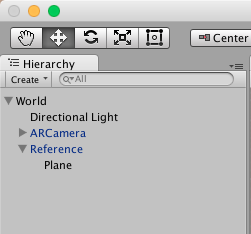
\includegraphics[width=0.25\textwidth]{hierarchy}
\end{figure}

O primeiro elemento, \textit{World}, do qual todos os outros são filhos, é o 
responsável por conter dois \textit{scripts} de comportamentos específicos da 
aplicação. Um deles é o \textit{LoadDeck.cs} que fica responsável por ler o 
arquivo de configuração e preparar sessenta \textit{frame markers} com as cartas 
do jogador. O outro é o \textit{Configuration.cs} responsável por carregar todo 
tipo de configuração que possa ser alterada pelo jogador antes de executar a 
aplicação. Por exemplo, o endereço na internet, IP, do adversário é carregado 
por este \textit{script}.

O segundo elemento, a \textit{Directional Light}, é um objeto que vem por padrão 
nas cenas assim que o Unity as cria. Nenhuma configuração adicional foi feita 
neste objeto.

O terceiro elemento, a \textit{AR Camera}, é um \textit{prefab} importado do 
Vuforia. Nele foi configurada a \textit{API Key} da aplicação. Sem esta 
informação, a ARCGP não seria capaz de utilizar a biblioteca de Realidade 
Aumentada. Também neste objeto está o \textit{script} de comportamento \textit{
NetworkEnvironmentShare.cs}. Ele é responsável por toda a parte de comunicação 
e rede da aplicação. Esse \textit{script} será detalhado na seção seguinte.

Por fim, tem-se o objeto chamado de \textit{Reference}. Esse pode ser chamado de 
um objeto coringa, pois no seu lugar pode-se ser colocado qualquer \textit{
prefab} rastreável desde que se substitua o \textit{script} de comportamento 
\textit{DefaultTrackableEventHandler.cs}, que é padrão da biblioteca Vuforia, 
pelo \textit{script ReferenceEnvironmentTracker.cs}. O comportamento que esse 
\textit{script} está responsável por enforçar será detalhado na seção seguinte.

No exemplo testado, foi utilizado um alvo de marcador comum, mas o usuário pode 
alterar esse objeto colocando um \textit{Image Target prefab} e utilizar uma 
imagem de sua escolha e possibilitar um \textit{extended tracking}, por exemplo.

\subsection{\textit{Scripts} de comportamento}
\label{scripts}
Foram preparados cinco \textit{scripts}, na linguagem C\# para implementar as 
funcionalidades previstas pelo projeto da ARCGP. Estes serão descritos em 
detalhes nesta seção.

\subsubsection{Configuration.cs}
\label{config}
Apesar de ser uma classe que estende \textit{MonoBehaviour} \cite{mono}, este 
\textit{script} existe para manter as variáveis que devem ser alteradas pelo 
usuário em um único local. Essas variáveis são: o IP do adversário, informação 
necessária para se conectar ao dispositivo do outro jogador; e uma 
\textit{string} descrevendo o \textit{deck} de cartas do jogador. O 
\textit{deck} descrito no arquivo \textit{Configuration.cs} no formato 
\textit{string} de identificação da carta, seguido por uma vírgula e, então, o 
número de de cópias daquela carta no \textit{deck}. A identificação da carta 
corresponde ao nome do arquivo de imagem da carta presente na pasta 
\textit{Resources}.

\subsubsection{LoadDeck.cs}
\label{loadeck}
Como foi explicado brevemente na seção anterior, esse \textit{script} é o 
responsável por ler, validar e carregar o \textit{deck} de cartas do jogador.
Quando as cartas são carregadas, o efeito é a adição de novos 
\textit{frame markers}, com objetos planos como seus filhos. Para cada plano 
corresponde uma carta, que é colocada como sua textura. A figura \ref{cardsld} 
mostra como deve ficar a hierarquia dos objetos depois que o \textit{deck} de 
cartas é carregado por este \textit{script}.

\begin{figure}[t]
	\caption{Hierarquia da Cena 3D após o carregamento do \textit{deck}
		 de cartas}
	\label{cardsld}
	\centering
	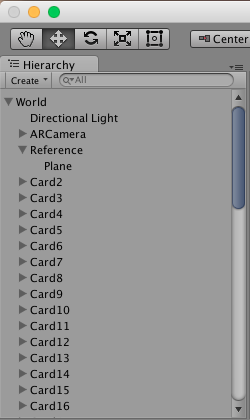
\includegraphics[width=0.25\textwidth]{hierarchyloaded}
\end{figure}

\subsubsection{CardTrackableEventHandler.cs}
\label{cardtracker}
Este \textit{script} é o substituto do \textit{DefaultTrackableEventHandler.cs} 
para marcadores de carta. Este comportamento é adicionado aos 
\textit{frame markers} assim que são adicionados à cena no \textit{script} 
mencionado na seção \ref{loadeck}. Contudo, ele não é tão diferente do 
\textit{script} padrão, pois apenas expõe o \textit{status} do rastreamento 
como atributo público da classe. Esse atributo é utilizado por outros 
\textit{scripts} para verificar se a carta deve ser mostrada também na cena do 
adversário.

\subsubsection{NetworkEnvironmentShare.cs}
\label{networkenv}
Este comportamento fica adicionado à câmera do jogo e é o responsável por toda 
a parte de conexão de rede entre os dois jogadores.

A maior preocupação deste \textit{script} é manter as atividades de rede em 
outras \textit{threads}, de forma que a comunicação ocorra de forma assíncrona 
com relação à \textit{thread} principal do jogo que atualiza a cena. De fato, o 
Unity não permite que \textit{threads} fora da principal utilize os recursos de 
sua API \cite{multithreading}.

Outra preocupação é implementar a comunicação em uma arquitetura \textit{
Peer-to-Peer} (P2P) \cite{p2p}, pois um servidor para servir de intermediário 
entre os dois jogadores não deveria ser requisito para que a aplicação 
funcionasse. Portanto, duas instâncias da aplicação devem funcionar, do ponto de 
vista de redes de computadores, como cliente e servidor ao mesmo tempo. Cada um 
desses papéis sendo executada em uma \textit{thread} diferente. Uma para escutar 
a porta do servidor, esperando por novas mensagens vindas do adversário e uma 
\textit{thread} para enviar mensagens geradas pelo \textit{script} do 
referencial, tratado na subseção seguinte.

Este \textit{script} mantém duas estruturas de dados do tipo FIFO (\textit{First 
In, First Out}) \cite{fifo}, uma para as mensagens recebidas pela conexão com o 
adversário, outra para enfileirar as mensagens a serem enviadas para o 
dispositivo adversário. As duas \textit{threads}, já mencionadas, se mantêm em 
\textit{loop} verificando se há novas mensagens enfileiradas (para a 
\textit{thread} responsável por enviar mensagens) ou se há mensagens no 
\textit{stream} de dados da rede (para a \textit{thread} responsável por receber 
mensagens).

As demais classes da aplicação, que são executadas na \textit{thread} principal 
do Unity, alimentam e consumem essas filas de mensagens.

\subsubsection{ReferenceEnvironmentTracker.cs}
\label{referencetrack}
Por fim, esse \textit{script} implementa duas tarefas: identificar o tabuleiro 
do jogo e verificar quais cartas estão na mão do jogador e quais estão em jogo.

A diferença está no fato de que, apesar de ambas precisarem ser exibidas na 
cena, sobre os marcadores, quando forem rastreadas, apenas as cartas em jogo 
devem ser enviadas para o adversário visualizar.

Esta distinção é feita da seguinte forma: as cartas que estiverem sendo 
rastreadas ao mesmo tempo que o marcador referencial devem estar em jogo. 
Enquanto que as cartas que estiverem sendo rastreadas sem o referencial, devem 
estar na mão do jogador. Além disso, se o referencial está sendo rastreado, e 
uma das cartas que estava em jogo não está mais sendo rastreada, então ela 
deve ter sido removida de jogo, seja qual for o seu destino.

Este \textit{script} pode enfileirar dois tipos de mensagens: uma mensagem com 
código \textit{see}, que significa que o adversário deve ver a carta passada 
como parâmetro, ou com código \textit{unsee}, que significa que o adversário 
deve parar de enxergar a carta passada como parâmetro. Como mencionado, 
a mensagem de código \textit{see} deve ter como parâmetro a carta a ser 
visualizada, mas além deste, devem ser informadas a posição e a rotação com as 
quais a carta deve ser desenhada na cena de destino.

Por fim, é também de responsabilidade desse \textit{script} verificar a fila de 
mensagens recebidas e adicionar as cartas especificadas como parâmetro, nas 
posição e rotação requisitadas e colocá-las como seus filhos dentro da 
hierarquia de objetos do Unity para que elas somente sejam exibidas quando ele 
estiver sendo rastreado (\textit{extended tracking} também é possível).

\section{Resultados}
\label{resultados}
Uma vez que a plataforma foi desenvolvida e testada, o resultado observado foi 
a satisfação dos requisitos elencados na seção \ref{objetivo}.

Um pequeno problema de usabilidade observado para o usuário leigo é a 
necessidade de configuração, do IP do adversário e do \textit{deck} de cartas, 
antes de compilar a aplicação, seja para Android \cite{android} ou para Desktop. 
O jogador também precisa imprimir os marcadores, disponibilizados no site do 
Vuforia, e recortá-los para utilizá-los no jogo.

Exportando para a plataforma Android \cite{android}, ao rodar o aplicativo, a 
aplicação irá imediatamente tentar conectar o dispositivo com o do jogador 
adversário. O jogador pode posicionar o marcador com identificador 1 no centro 
da superfície onde deseja jogar. A partir de então, basta posicionar os 
marcadores na superfície quando desejar colocar as respectivas cartas em jogo e 
prosseguir com a partida como faria com o jogo tradicional.

Foram separadas algumas imagens, tiradas diretamente dos dispositivos, que 
ilustram brevemente a aplicação sendo executada.

A figura \ref{owntablereal} mostra um possível tabuleiro sem os objetos virtuais 
adicionados pela aplicação, ou seja, trata-se de uma imagem puramente real.

\begin{figure}[b]
	\caption{Tabuleiro visualizado sem a aplicação de realidade aumentada}
	\label{owntablereal}
	\centering
	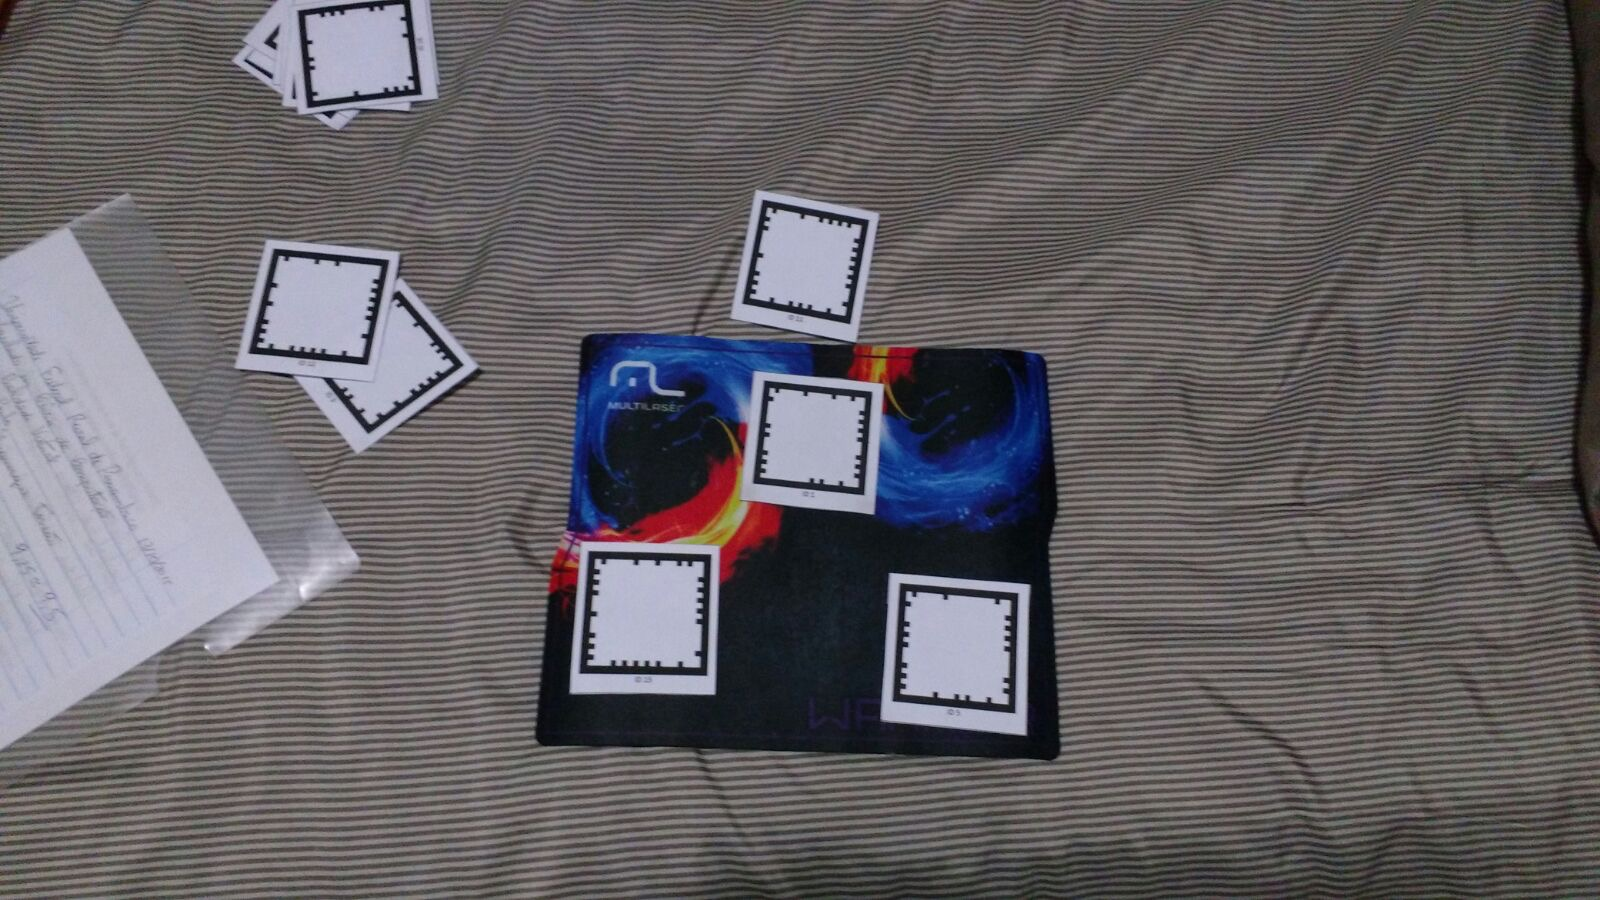
\includegraphics[width=0.25\textwidth]{owntablereal}
\end{figure}

A figura \ref{owntableaug}, por sua vez, mostra o mesmo momento com a realidade 
aumentada. Note que tanto esta figura quanto a figura \ref{owntablereal} não 
possuem cartas do adversário transmitidas para o tabuleiro mostrado.

Por fim, a figura \ref{enemytable} mostra um tabuleiro com três cartas virtuais 
sendo exibidas. É importante notar que o cenário dessa figura não é o mesmo 
mostrado nesta figura.

\section{Trabalhos Futuros}
\label{trab_fut}
Nesta seção, serão apresentadas algumas possíveis melhorias para a plataforma
proposta. Estas não foram implementadas neste primeiro momento por não terem 
sido previstas no planejamento e por conta da restrições no cronograma.

Em um primeiro momento, seria importante se dedicar à simplificação da 
arquitetura da plataforma. É possível modificar os \textit{scripts} de 
comportamento que foram desenvolvidos para que fiquem menos interligados à API 
do Vuforia, tornando-os mais modulares e criando mais oportunidades de reuso do 
código.

Foi verificado, durante os testes, que um esquema mais sofisticado para 
identificação de quais cartas estão em jogo e quais ainda não foram jogadas, por 
parte da aplicação, aumentaria a jogabilidade. Um possível esquema seria adição 
de mais um marcador ao qual não estaria associado nenhuma carta. Esse marcador 
funcionaria de forma similar ao Referencial descrito na seção \ref{plataforma}: 
os \textit{frame markers}, associados a cartas, que estivessem sendo rastreados 
ao mesmo tempo que este novo marcador seriam consideradas como estando na 
mão do jogador. Isso ajudaria a aplicação a ter uma contagem das cartas na mão 
do jogador e poderia transmitir essa informação para o adversário, pois ela é 
importante em alguns jogos de cartas.

Por fim, poderia-se criar uma aplicação exclusiva para o jogo \textit{Magic: The 
Gathering}. Essa aplicação poderia implementar regras de jogo para garantir a um 
jogador que seu adversário não está agindo de forma ilegal. Isso no entanto, 
adiciona complexidade para o entendimento da aplicação por parte do usuário e 
remove um pouco da sua familiaridade com a forma de jogar.

\section{Conclusão}
\label{conclusao}
Neste artigo, foi descrito o projeto da ARCGP, uma plataforma para jogos de 
cartas com realidade aumentada. Primeiramente foi apresentada uma falta de 
trabalhos com a preocupação de possibilitar o jogo de cartas de forma remota e 
se valendo da realidade aumentada para manter a familiaridade da mecânica de 
jogo. Os trabalhos encontrados com maior similaridade foram descritos e as 
diferenças para a ARCGP foram esclarecidas.

\begin{figure}[t]
	\caption{Tabuleiro visualizado com a aplicação de realidade aumentada}
	\label{owntableaug}
	\centering
	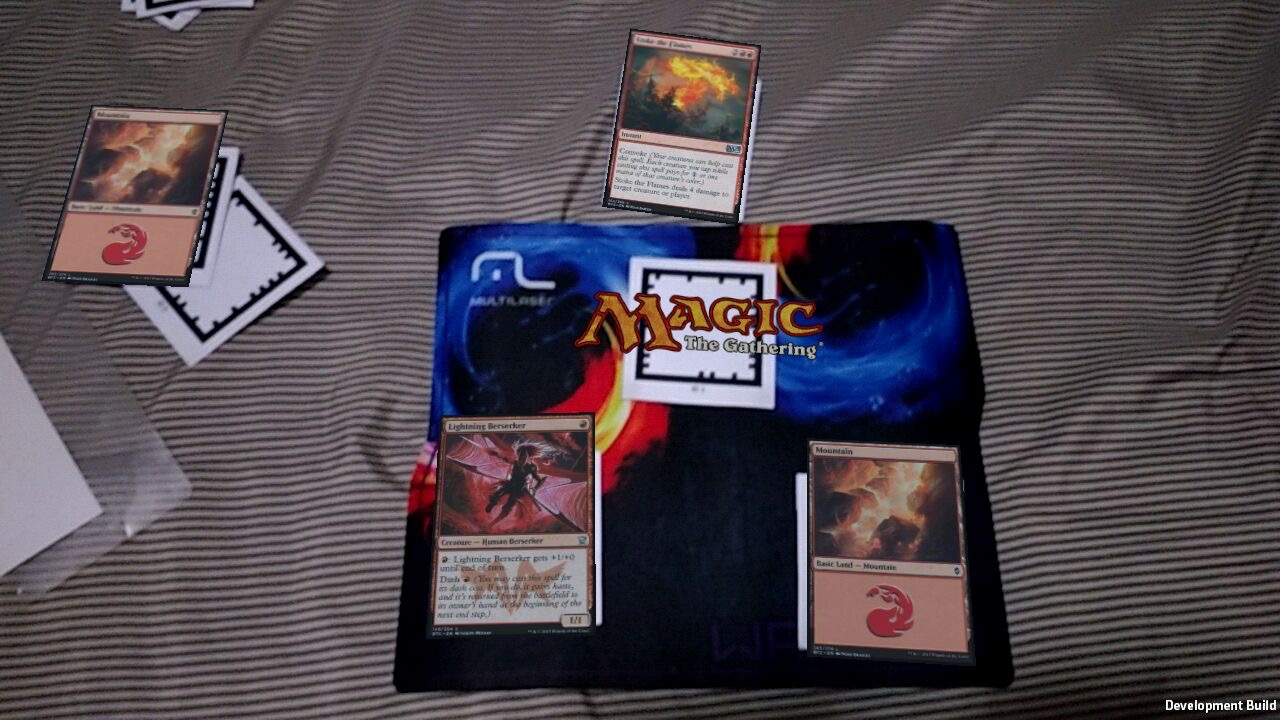
\includegraphics[width=0.25\textwidth]{owntableaug}
\end{figure}

Depois de descrever os objetivos e a metodologia, este artigo descreveu, com 
riqueza de detalhes, a implementação da plataforma utilizando o motor de jogos, 
Unity, com a API do Vuforia.

Em seguida foram descritas e ilustradas as capacidades da aplicação 
desenvolvida, bem como suas limitações.

Por fim, foram apresentados trabalhos a serem feitos para incrementar a 
plataforma e a aplicação.

A plataforma proposta e implementada se mostrou capaz de auxiliar jogadores 
a jogarem jogos de cartas sem precisarem se deslocar. Além disso, a aplicação 
resultante é uma alternativa prática para os jogadores, já que pode ser baixada 
e compilada para seus celulares portáteis. Assim, ela é de baixo custo e não 
necessita de aparelhos, ferramentas ou dispositivos com dificuldades de 
aquisição e mobilidade.

\begin{figure}[t]
	\caption{Tabuleiro visualizado pelo jogador com realidade aumentada. Note 
		que as três cartas exibidas são provenientes do adversário, já que não 
		há marcadores para elas sendo rastreados.}
	\label{enemytable}
	\centering
	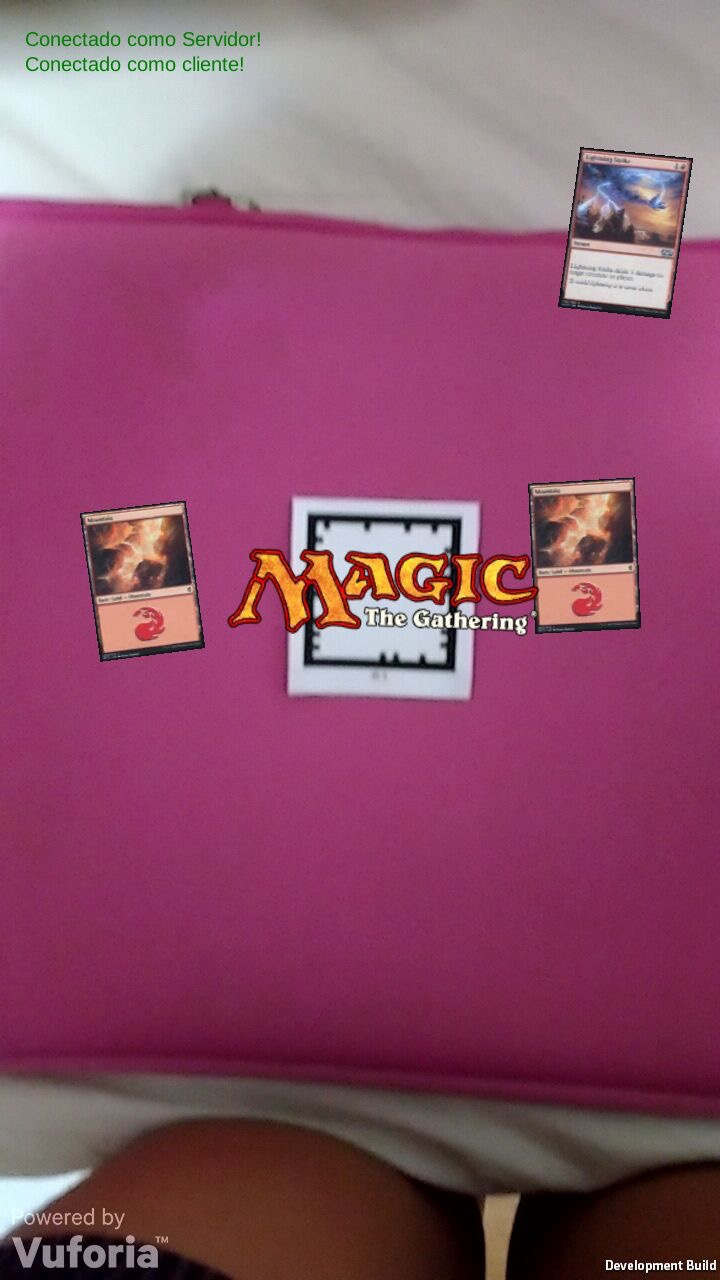
\includegraphics[width=0.25\textwidth]{enemytable}
\end{figure}

\bibliographystyle{IEEEtran}
\bibliography{bibi}
\end{document}